% ===== Block 1: Docker Compose (slides 5-36) =====
\sectionframe{Docker Compose}

% --- What is Docker Compose? ---
\begin{frame}{What is Docker Compose?}
  \begin{itemize}
    \item Compose is a layer ``on top'' of Docker
    \item Docker compose allows to
      \begin{itemize}
        \item \textbf{Combine} multiple containers that interact with each other
        \item Start / Stop multiple containers easily
        \item \textbf{Persist} data in volumes
        \item Configure multiple \textbf{isolated environments} (e.g.\ development and testing)
        \item \textbf{Deploy} software to a Server / VM
      \end{itemize}
  \end{itemize}
\end{frame}

% --- The Docker Compose File ---
\begin{frame}{The Docker Compose File}
  \begin{itemize}
    \item Docker compose files are written in \textbf{yaml}: \texttt{compose.yaml}
    \item Defining:
      \begin{itemize}
        \item \texttt{services}
          \begin{itemize}
            \item Abstraction of a computing resource
            \item A valid \texttt{compose.yaml} has to specify at least one service
          \end{itemize}
        \item \texttt{networks}
          \begin{itemize}
            \item Abstraction of a communication channel
            \item Handle service discovery
          \end{itemize}
        \item \texttt{volumes} / \texttt{configs} / \texttt{secrets}
      \end{itemize}
  \end{itemize}
\end{frame}

% --- Example: services (2 bubbles) ---
\begin{frame}[fragile]{Example: \texttt{services}}
  Create a \texttt{compose.yml} file:
  \begin{yamlbox}
\begin{lstlisting}[style=wsyamlstyle]
services:
  (*\tikzmark{s8app}*)app:
    (*\tikzmark{s8img}*)image: "hello-world"
\end{lstlisting}
  \end{yamlbox}
  \medskip Start the compose with
  \begin{termbox}
\begin{lstlisting}[style=wstermstyle]
~/workshop> docker compose up
\end{lstlisting}
  \end{termbox}
  \begin{tikzpicture}[remember picture, overlay]
    \bubbleat{\pg{9.3cm}{-2.55cm}}{s8app}{We create a \texttt{service} called ``app''}
    \bubbleat{\pg{9.3cm}{-3.7cm}}{s8img}{From the \texttt{image} ``hello-world''}
  \end{tikzpicture}
\end{frame}

% --- Example: Multiple services (2 bubbles to terminals) ---
\begin{frame}[fragile]{Example: Multiple \texttt{services}}
  Update the \texttt{compose.yml} file:
  \begin{yamlbox}
\begin{lstlisting}[style=wsyamlstyle]
services:
  app1:
    image: "nginxdemos/hello"
  app2:
    image: "nginxdemos/hello"
\end{lstlisting}
  \end{yamlbox}
  \medskip Start the compose with
  \begin{termbox}
\begin{lstlisting}[style=wstermstyle]
~/workshop> docker compose up (*\tikzmark{s9det}*)-d
\end{lstlisting}
  \end{termbox}
  \smallskip
  \begin{termbox}
\begin{lstlisting}[style=wstermstyle]
~/workshop> docker compose (*\tikzmark{s9ps}*)ps
\end{lstlisting}
  \end{termbox}
  \begin{tikzpicture}[remember picture, overlay]
    \bubbleat{\pg{10cm}{-4.3cm}}{s9det}{The containers now run in the background (``detached'')}
    \bubbleat{\pg{10cm}{-5.8cm}}{s9ps}{Shows the running containers}
  \end{tikzpicture}
\end{frame}

% --- docker compose ps ---
\begin{frame}[fragile]{\texttt{docker compose ps}}
  Initial version of our \texttt{compose.yaml}:
  \begin{termbox}
\begin{lstlisting}[style=wstermstyle, basicstyle=\ttfamily\scriptsize\color{wsgreen}]
~/workshop> docker compose ps
NAME             IMAGE             SERVICE      STATUS        PORTS
serverside1-1    nginxdemos/hello  serverside1  Up 3 minutes  80/tcp
serverside2-1    nginxdemos/hello  serverside2  Up 3 minutes  80/tcp
\end{lstlisting}
  \end{termbox}
  \begin{itemize}
    \item The containers offer port 80 - but we can't access it yet
  \end{itemize}
\end{frame}

% --- Example: Make services accessible (1 bubble) ---
\begin{frame}[fragile]{Example: Make \texttt{services} accessible}
  Update the \texttt{compose.yml} file:
  \begin{yamlbox}
\begin{lstlisting}[style=wsyamlstyle]
services:
  app1:
    image: "nginxdemos/hello"
    ports:
      (*\tikzmark{s11p}*)- "8081:80"
  app2:
    image: "nginxdemos/hello"
    ports:
      - "8082:80"
\end{lstlisting}
  \end{yamlbox}
  \begin{tikzpicture}[remember picture, overlay]
    \bubbleat{\pg{9.6cm}{-4.4cm}}{s11p}{We map the host port 8081 to the container port 80}
  \end{tikzpicture}
\end{frame}

% --- Example: Inspect our services (screenshots) ---
\begin{frame}{Example: Inspect our \texttt{services}}
  \begin{itemize}\item Each container has an (unique) IP address\end{itemize}
  \vfill\centering
  \begin{columns}[c]
    \column{0.46\textwidth}\centering\removedimage{nginx demo page \\ (shows 172.20.0.2:80)}
    \column{0.46\textwidth}\centering\removedimage{nginx demo page \\ (shows 172.20.0.3:80)}
  \end{columns}
  \vfill
\end{frame}

% --- Configure Containers: environment (1 bubble) ---
\begin{frame}[fragile]{Configure Containers: \texttt{environment}}
  \begin{itemize}\item Inject variables into containers\end{itemize}
  \begin{yamlbox}
\begin{lstlisting}[style=wsyamlstyle]
services:
  app1:
    image: "nginxdemos/hello"
    ports:
      - "8080:80"
    (*\tikzmark{s14env}*)environment:
      - "SOME_KEY=SOME_VALUE"
\end{lstlisting}
  \end{yamlbox}
  \begin{itemize}
    \item Never put secrets directly into the compose file - Use \texttt{.env} files instead
    \item Applications need to handle environment variables!
  \end{itemize}
  \begin{tikzpicture}[remember picture, overlay]
    \bubbleat{\pg{9.6cm}{-4.6cm}}{s14env}{Never put secrets directly into the compose file - Use .env files instead}
  \end{tikzpicture}
\end{frame}

% --- Our Running Example: Pedelec App (photo placeholder) ---
\begin{frame}{Our Running Example: Pedelec App}
  \begin{columns}[c]
    \column{0.62\textwidth}
      Our office is located in close proximity to our customers. The access to
      public transportation is poor and the number of available parking spots at
      the customer's site is low.
      \medskip

      With a bike, the customer site is easy to reach and only minimal parking
      space is required. To reduce the commuting time to a minimum we plan to
      operate a pool of Pedelecs (electricity powered bicycles) for our employees.
      Pedelecs can be reserved with a new mobile app.
    \column{0.34\textwidth}
      \centering\removedimage{cyclist photo}
  \end{columns}
\end{frame}

% --- Our Running Example: Pedelec App (Marie story) ---
\begin{frame}{Our Running Example: Pedelec App}
  Marie, an Accenture employee in Munich, has an appointment at BMW's
  ``Forschungs- und Innovationszentrum''. BMW does not have enough public parking
  spots so she cannot use her car. If she uses a Pedelec the trip can be done in
  10 minutes.
  \medskip

  She searches for a Pedelec in her app and sees that 3 of them are available and
  have enough battery power to reach BMW. Marie reserves this Pedelec.
  \medskip

  When Marie arrives at the bike lot, the app automatically displays the PIN to
  unlock the Pedelec. She unlocks it and drives to BMW. There she notices that
  the bell of the bike is damaged. She reports this damage with the app. After
  she is back at Accenture, she returns the bike and releases her reservation.
\end{frame}

% --- Software Engineering Happening (meme placeholder) ---
\begin{frame}{Software Engineering Happening}
  \centering\vfill\removedimage{developer meme}\vfill
\end{frame}

% --- Pedelec Server Side (component diagram) ---
\begin{frame}{Pedelec Server Side}
  \centering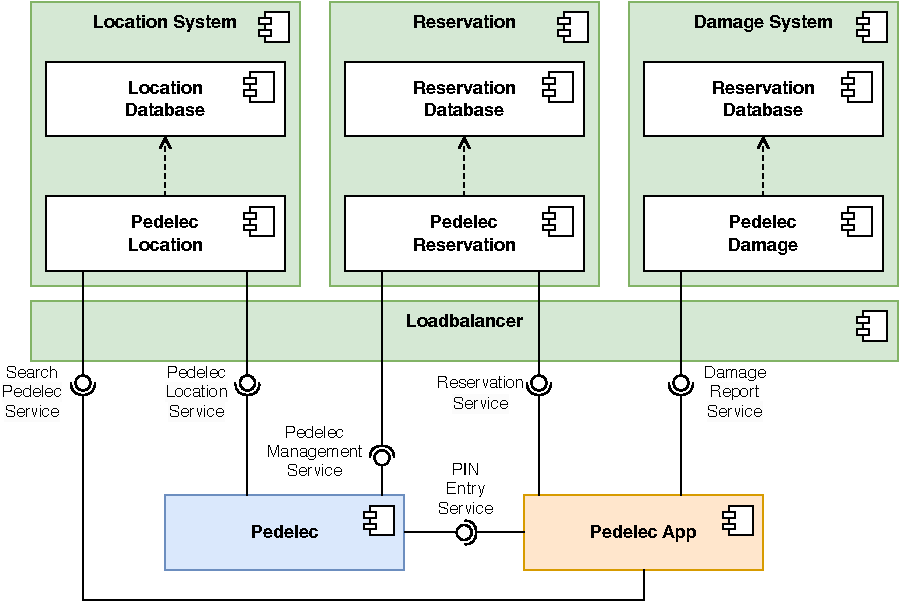
\includegraphics[height=0.74\paperheight]{assets/dia-pedelec-ssd.pdf}
\end{frame}

% --- Exercise: Pedelec App Overview ---
\begin{frame}{\exicon Exercise: Pedelec App Overview}
  \texttt{https://github.com/\wsImageOwner/kubernetes-workshop}
  \begin{itemize}
    \item Task 1: Fork and Clone the Pedelec Repo
    \item Task 2: Inspect the Server Side (\texttt{./exercises/01-microservices})
    \item Task 3: Start the Server Side with docker compose
  \end{itemize}
\end{frame}

% --- Tasks ---
\begin{frame}[fragile]{\exicon Tasks}
  \begin{termbox}
\begin{lstlisting}[style=wstermstyle]
git clone git@github.com:mtze/kubernetes-workshop.git
cd kubernetes-workshop/exercises/01-microservices
docker compose up
\end{lstlisting}
  \end{termbox}
\end{frame}

% --- Exercise: Pedelec App API ---
\begin{frame}{\exicon Exercise: Pedelec App API}
  \begin{enumerate}
    \item Task 1: Open Bruno
    \item Task 2: Open the Bruno config
    \item Task 3: Check if the API is working
  \end{enumerate}
\end{frame}

% --- The Docker Compose File (revisited) ---
\begin{frame}{The Docker Compose File}
  \begin{itemize}
    \item Docker compose files are written in \textbf{yaml}: \texttt{compose.yaml}
    \item Defining:
      \begin{itemize}
        \item \texttt{services} {\color{wsstr}$\checkmark$}
          \begin{itemize}
            \item Abstraction of a computing resource
            \item A valid \texttt{compose.yaml} has to specify at least one service
          \end{itemize}
        \item \texttt{networks}
          \begin{itemize}
            \item Abstraction of a communication channel
            \item Handle service discovery
          \end{itemize}
        \item \texttt{volumes} / \texttt{configs} / \texttt{secrets}
      \end{itemize}
  \end{itemize}
\end{frame}

% --- Example: networks (diagrams) ---
\begin{frame}{Example: \texttt{networks}}
  \begin{itemize}\item Architecture we created with \texttt{ports}\end{itemize}
  \begin{center}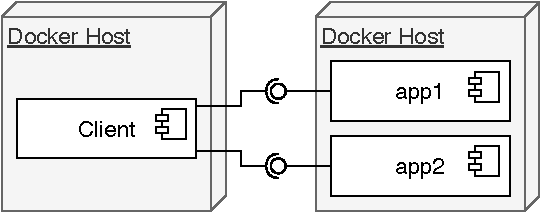
\includegraphics[height=0.26\paperheight]{assets/dia-net-port.pdf}\end{center}
  \begin{itemize}\item Architectures we can create with \texttt{networks}\end{itemize}
  \begin{center}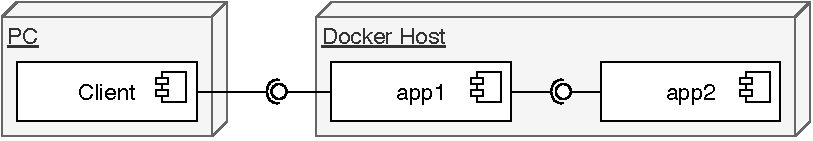
\includegraphics[height=0.26\paperheight]{assets/dia-net-network.pdf}\end{center}
\end{frame}

% --- Example: Create networks (4 bubbles) ---
\begin{frame}[fragile]{Example: Create \texttt{networks}}
  \begin{columns}[T]
    \column{0.52\textwidth}
      Update the \texttt{compose.yml} file:
      \begin{yamlbox}
\begin{lstlisting}[style=wsyamlstyle, basicstyle=\ttfamily\scriptsize]
services:
  app1:
    image: "nginxdemos/hello"
    (*\tikzmark{n1}*)ports:
      - "8080:80"
    (*\tikzmark{n2}*)networks:
      - mynet
  app2:
    image: "nginxdemos/hello"
    networks:
      - mynet
    (*\tikzmark{n3}*)expose:
      - "80"
(*\tikzmark{n4}*)networks:
  mynet:
\end{lstlisting}
      \end{yamlbox}
    \column{0.46\textwidth}
  \end{columns}
  \begin{tikzpicture}[remember picture, overlay]
    \bubbleat{\pg{10.5cm}{-2.1cm}}{n1}{We're still using \texttt{ports} to map the service to the host}
    \bubbleat{\pg{10.5cm}{-3.5cm}}{n2}{Both containers connect to the same network}
    \bubbleat{\pg{10.5cm}{-5.0cm}}{n3}{We replaced the \texttt{port} mapping with an \texttt{expose} to limit access to the ``mynet'' network}
    \bubbleat{\pg{10.5cm}{-6.6cm}}{n4}{We explicitly define a \texttt{network}}
  \end{tikzpicture}
\end{frame}

% --- docker compose ps (networks) ---
\begin{frame}[fragile]{\texttt{docker compose ps}}
  Updated \texttt{compose.yaml} with a private network:
  \begin{termbox}
\begin{lstlisting}[style=wstermstyle, basicstyle=\ttfamily\scriptsize\color{wsgreen}]
~/workshop> docker compose ps
NAME       IMAGE             SERVICE  STATUS         PORTS
app1-1     nginxdemos/hello  app1     Up 15 seconds  0.0.0.0:8080->80/tcp
app2-1     nginxdemos/hello  app2     Up 15 seconds  80/tcp
\end{lstlisting}
  \end{termbox}
  \begin{itemize}
    \item app1 is reachable from outside the network: \texttt{port}
    \item app2 is only reachable from within the network: \texttt{expose}
  \end{itemize}
\end{frame}

% --- Useful commands ---
\begin{frame}[fragile]{Useful commands}
  \begin{termbox}
\begin{lstlisting}[style=wstermstyle, basicstyle=\ttfamily\scriptsize\color{wsgreen}]
docker compose up       # Starts the project in foreground
docker compose up -d    # Starts the project in the background
docker compose ps       # Shows all running services
docker compose down     # Stops the project
docker compose logs     # Shows the logs of all containers
docker compose pull     # Pulls the images of all services
\end{lstlisting}
  \end{termbox}
\end{frame}

\breakframe

% ===== Scaling & Load Balancing =====
\sectionframe{Scaling your Application}

% --- What is scaling? ---
\begin{frame}{What is scaling?}
  \orangeband{Scalability is the property of a system to handle a growing amount
  of work by adding resources to the system.}
  \begin{itemize}
    \item How can we scale?
      \begin{itemize}
        \item Make the existing resources more capable
        \item Add more of the same resources we have already
      \end{itemize}
  \end{itemize}
\end{frame}

% --- Scale up vs out: vertical (diagram) ---
\begin{frame}{Scale up vs.\ Scale out}
  \begin{columns}[c]
    \column{0.6\textwidth}
      \begin{itemize}
        \item \textbf{Vertical Scaling:} Scaling up / down
          \begin{itemize}
            \item Scale the machine (More CPU / More RAM)
            \item {\color{wsstr}\textbf{Benefits}}
              \begin{itemize}\item No software changes required \item Easy to maintain\end{itemize}
            \item {\color{red!70!black}\textbf{Drawbacks}}
              \begin{itemize}\item Limited by physics \item Hardware cost may be significant\end{itemize}
          \end{itemize}
      \end{itemize}
    \column{0.36\textwidth}
      \centering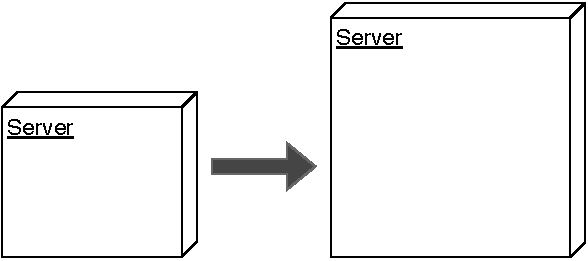
\includegraphics[width=\linewidth]{assets/dia-scale-up.pdf}
  \end{columns}
\end{frame}

% --- Scale up vs out: horizontal (diagram) ---
\begin{frame}{Scale up vs.\ Scale out}
  \begin{columns}[c]
    \column{0.6\textwidth}
      \begin{itemize}
        \item \textbf{Horizontal Scaling:} Scaling out / in
          \begin{itemize}
            \item Scale the application
            \item {\color{wsstr}\textbf{Benefits}}
              \begin{itemize}\item Flexible \item Limitless (More or less)\end{itemize}
            \item {\color{red!70!black}\textbf{Drawbacks}}
              \begin{itemize}\item More complex architecture \item Harder to debug\end{itemize}
          \end{itemize}
        \item If we talk about scaling today we mean horizontal scaling
      \end{itemize}
    \column{0.36\textwidth}
      \centering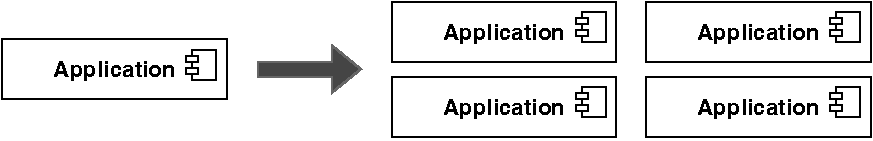
\includegraphics[width=\linewidth]{assets/dia-scale-out.pdf}
  \end{columns}
\end{frame}

% --- Scalable Architectures ---
\begin{frame}{Scalable Architectures}
  Key aspects for a scalable architecture:
  \begin{itemize}
    \item \textbf{API-First Design:} Clear interfaces between components
    \item \textbf{Stateless Services:} Design services to avoid local state
    \item \textbf{Async Communication:} Prefer message queues or event-driven designs
    \item \textbf{Database Sharding/Replication:} Avoid bottlenecks by scaling data layers
    \item \textbf{Observability and Monitoring:} Integrate logging, metrics, and tracing
    \item \textbf{Resilience and Fault Tolerance:} Retries, circuit breakers, graceful degradation
  \end{itemize}
\end{frame}

% --- Pedelec Server Side (scalability review) ---
\begin{frame}{Pedelec Server Side}
  \begin{columns}[c]
    \column{0.62\textwidth}
      \centering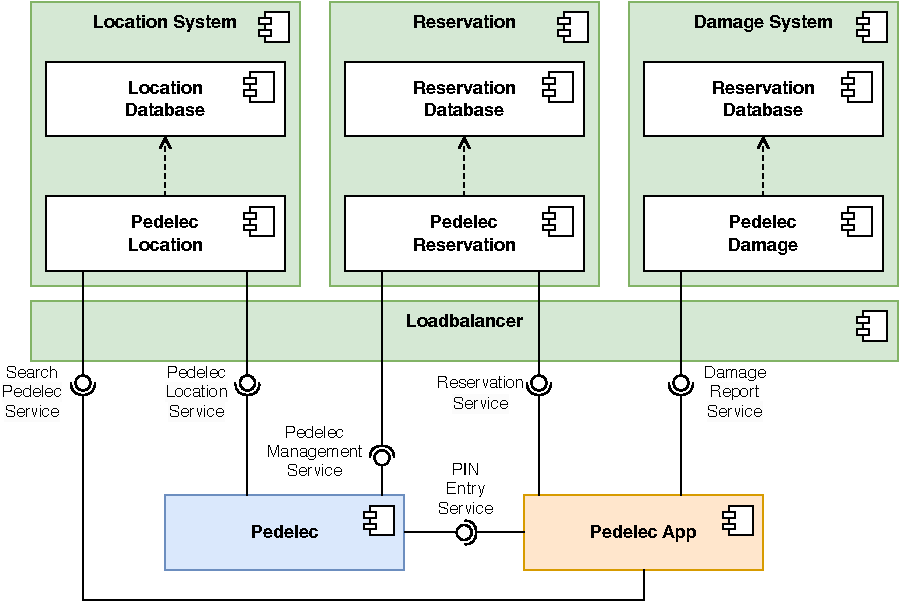
\includegraphics[width=\linewidth]{assets/dia-pedelec-ssd.pdf}
    \column{0.34\textwidth}
      Reviewing against the scalability aspects:
      \begin{itemize}
        \item DB Shards {\color{wsstr}$\checkmark$}
        \item Stateless Controller {\color{wsstr}$\checkmark$}
        \item API Specs {\color{wsstr}$\checkmark$}
        \item Event Framework?
      \end{itemize}
  \end{columns}
\end{frame}

% --- Problems with scaling ---
\begin{frame}{Problems with scaling}
  \begin{itemize}
    \item Service Discovery \item Load Balancing \item Shared Data
    \item Shared Storage \item Configuration Management \item Observability
  \end{itemize}
\end{frame}

% --- Load Balancing ---
\begin{frame}{Load Balancing}
  \orangeband{Load balancing is the process of distributing a set of tasks over
  a set of resources, with the aim of making their overall processing more efficient.}
  \begin{itemize}
    \item Load balancing can be conducted on \textbf{different levels}
    \item Example: University Assignments
      \begin{itemize}\item Distribute by exercise sheet \item Distribute by exercise \item Distribute by sub problem\end{itemize}
  \end{itemize}
\end{frame}

% --- ISO/OSI Model (self-contained diagram) ---
\begin{frame}{ISO/OSI Model}
  \vfill
  \centering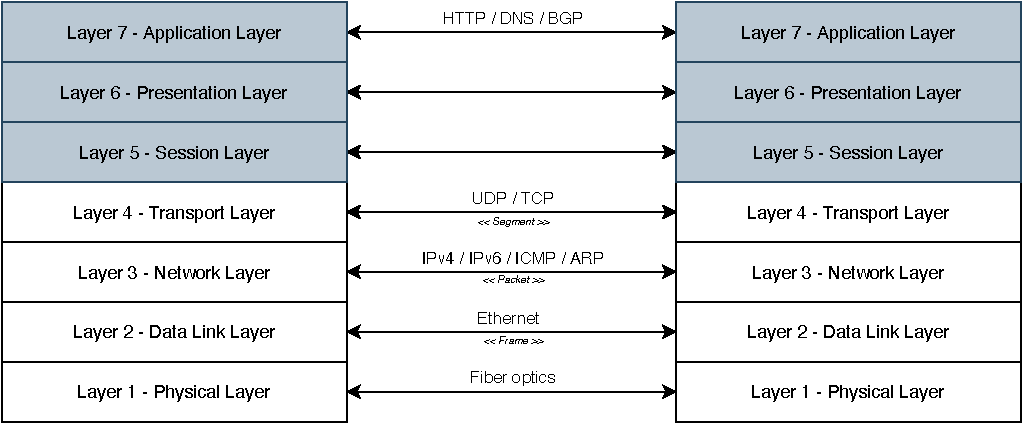
\includegraphics[width=\textwidth,height=0.72\paperheight,keepaspectratio]{assets/dia-osi.pdf}
  \vfill
\end{frame}
